\begin{figure}[htbp]
    \captionsetup[subfigure]{justification=centering}
    \centering
    \begin{subfigure}[b]{0.3\textwidth}
        \centering
        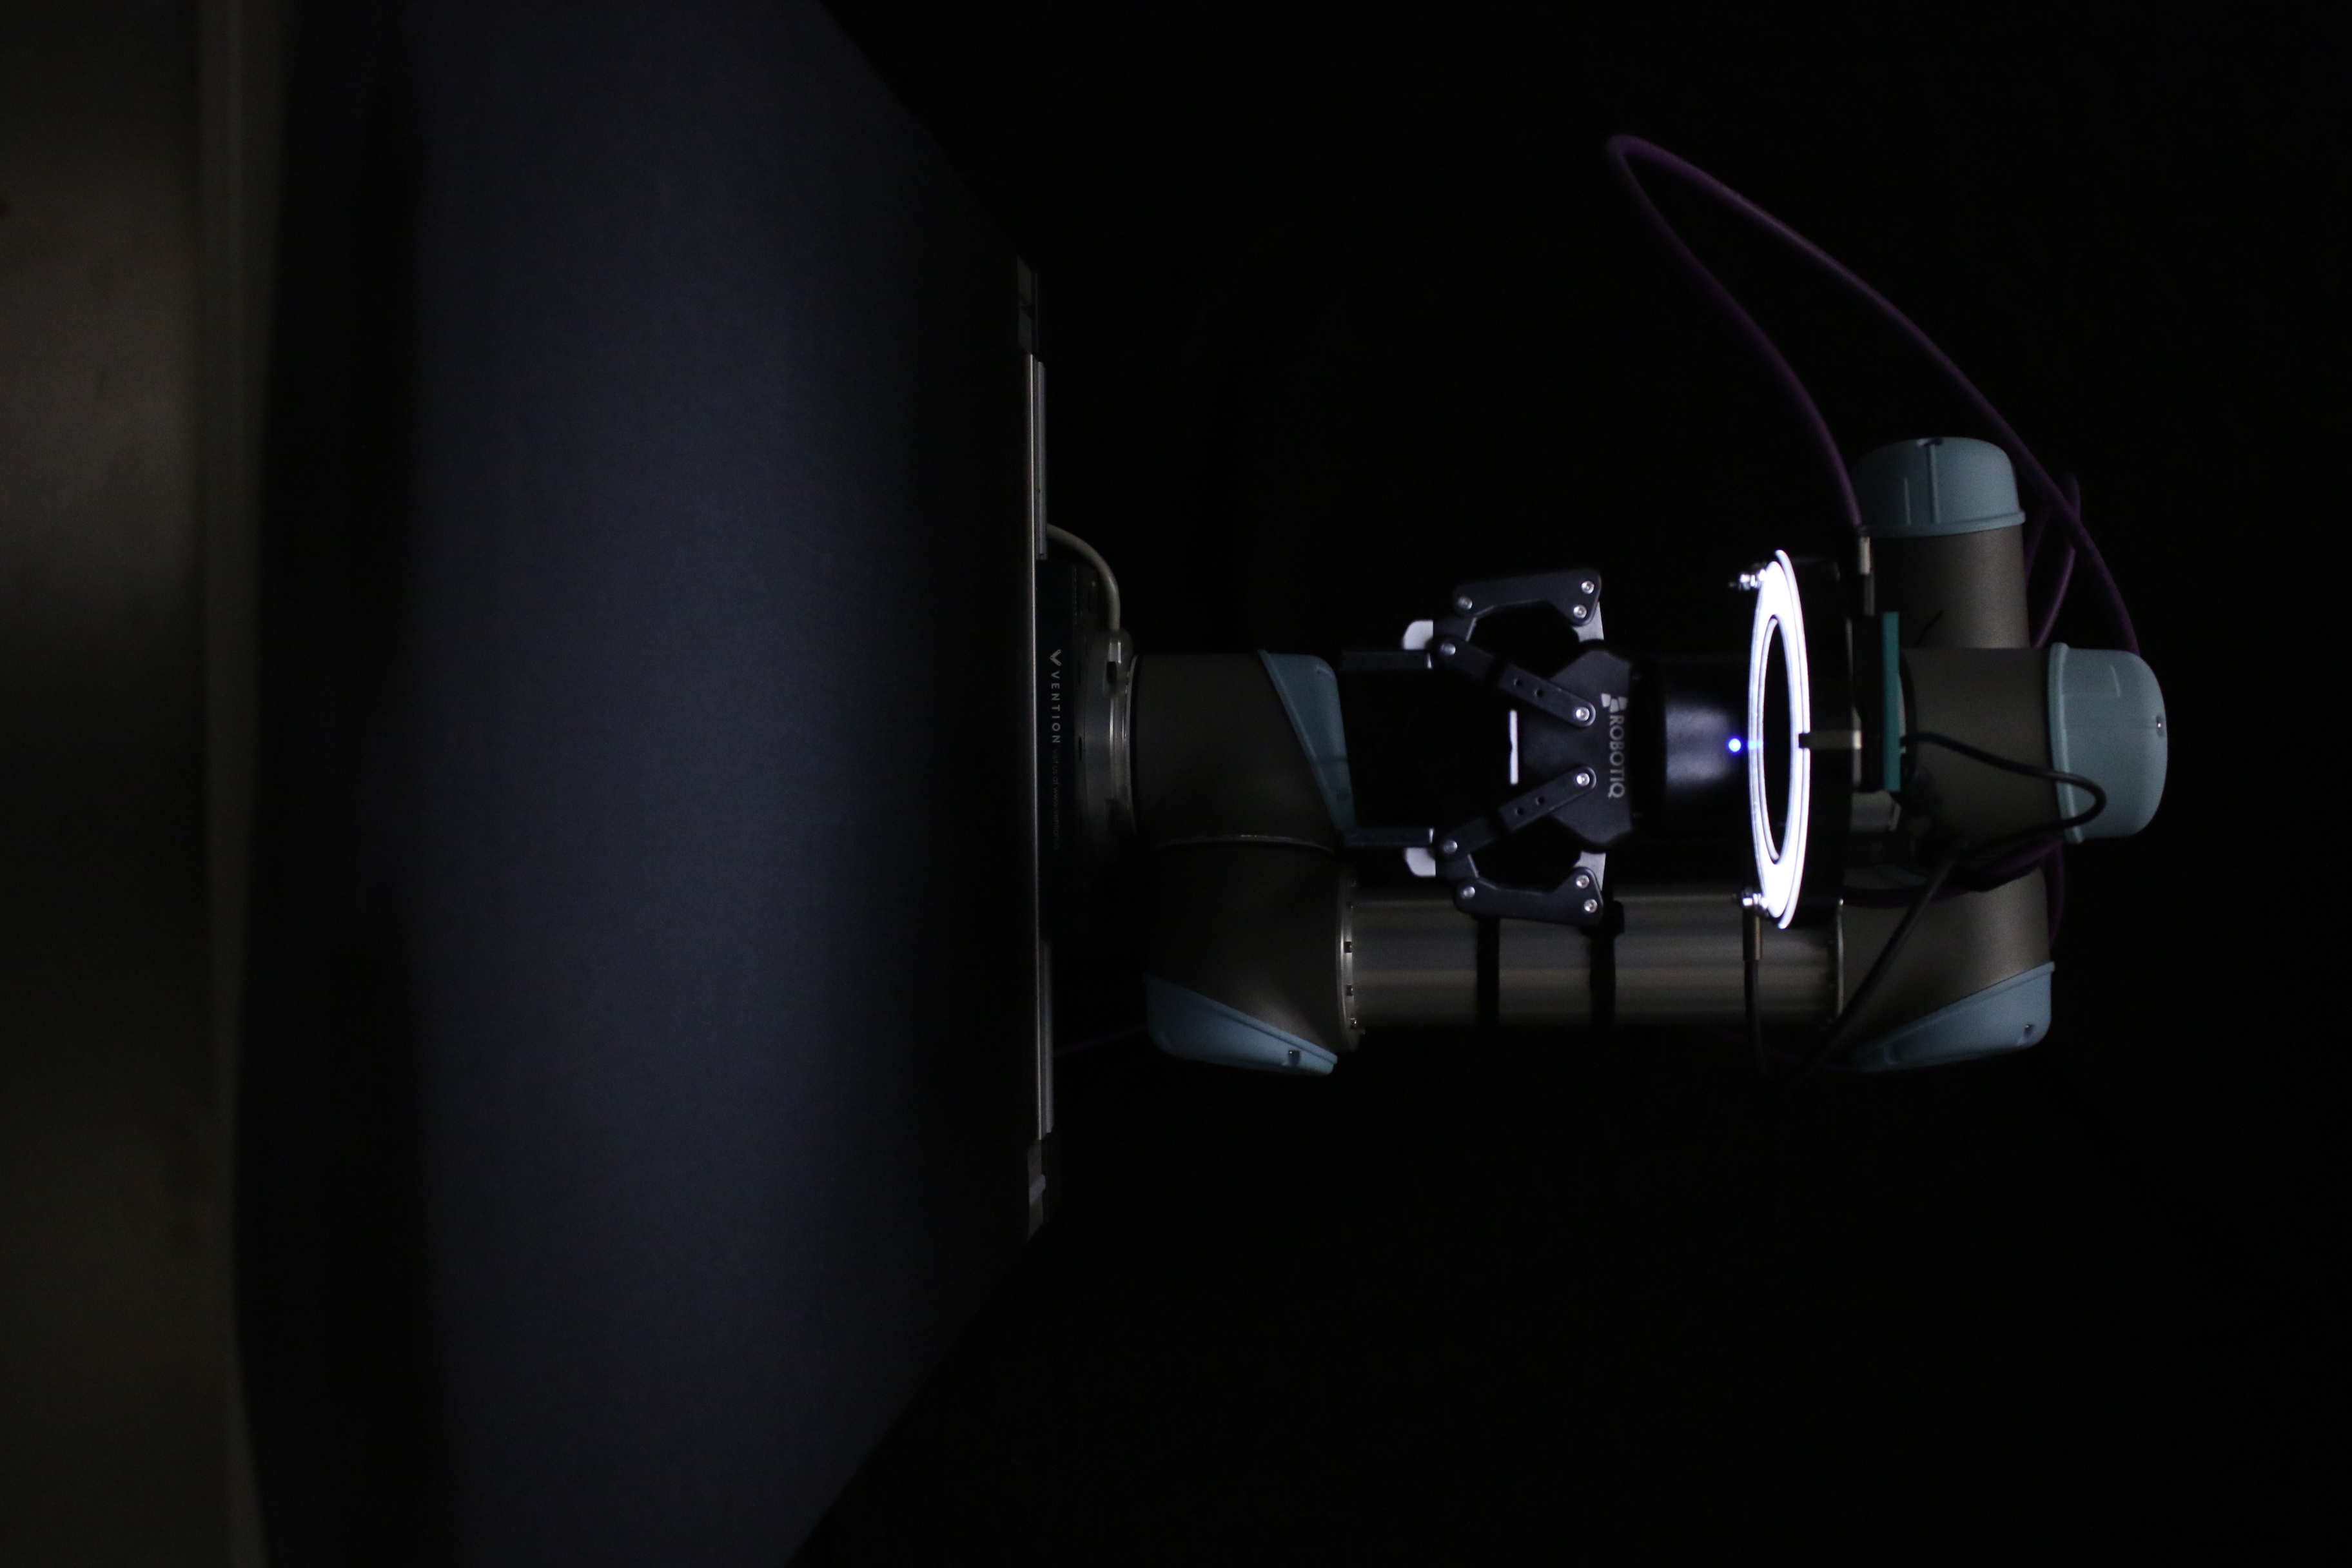
\includegraphics[angle=90, width=\textwidth]{figures/setupimages/setup_empty.JPG}


    \end{subfigure}
    \begin{subfigure}[b]{0.3\textwidth}
        \centering
        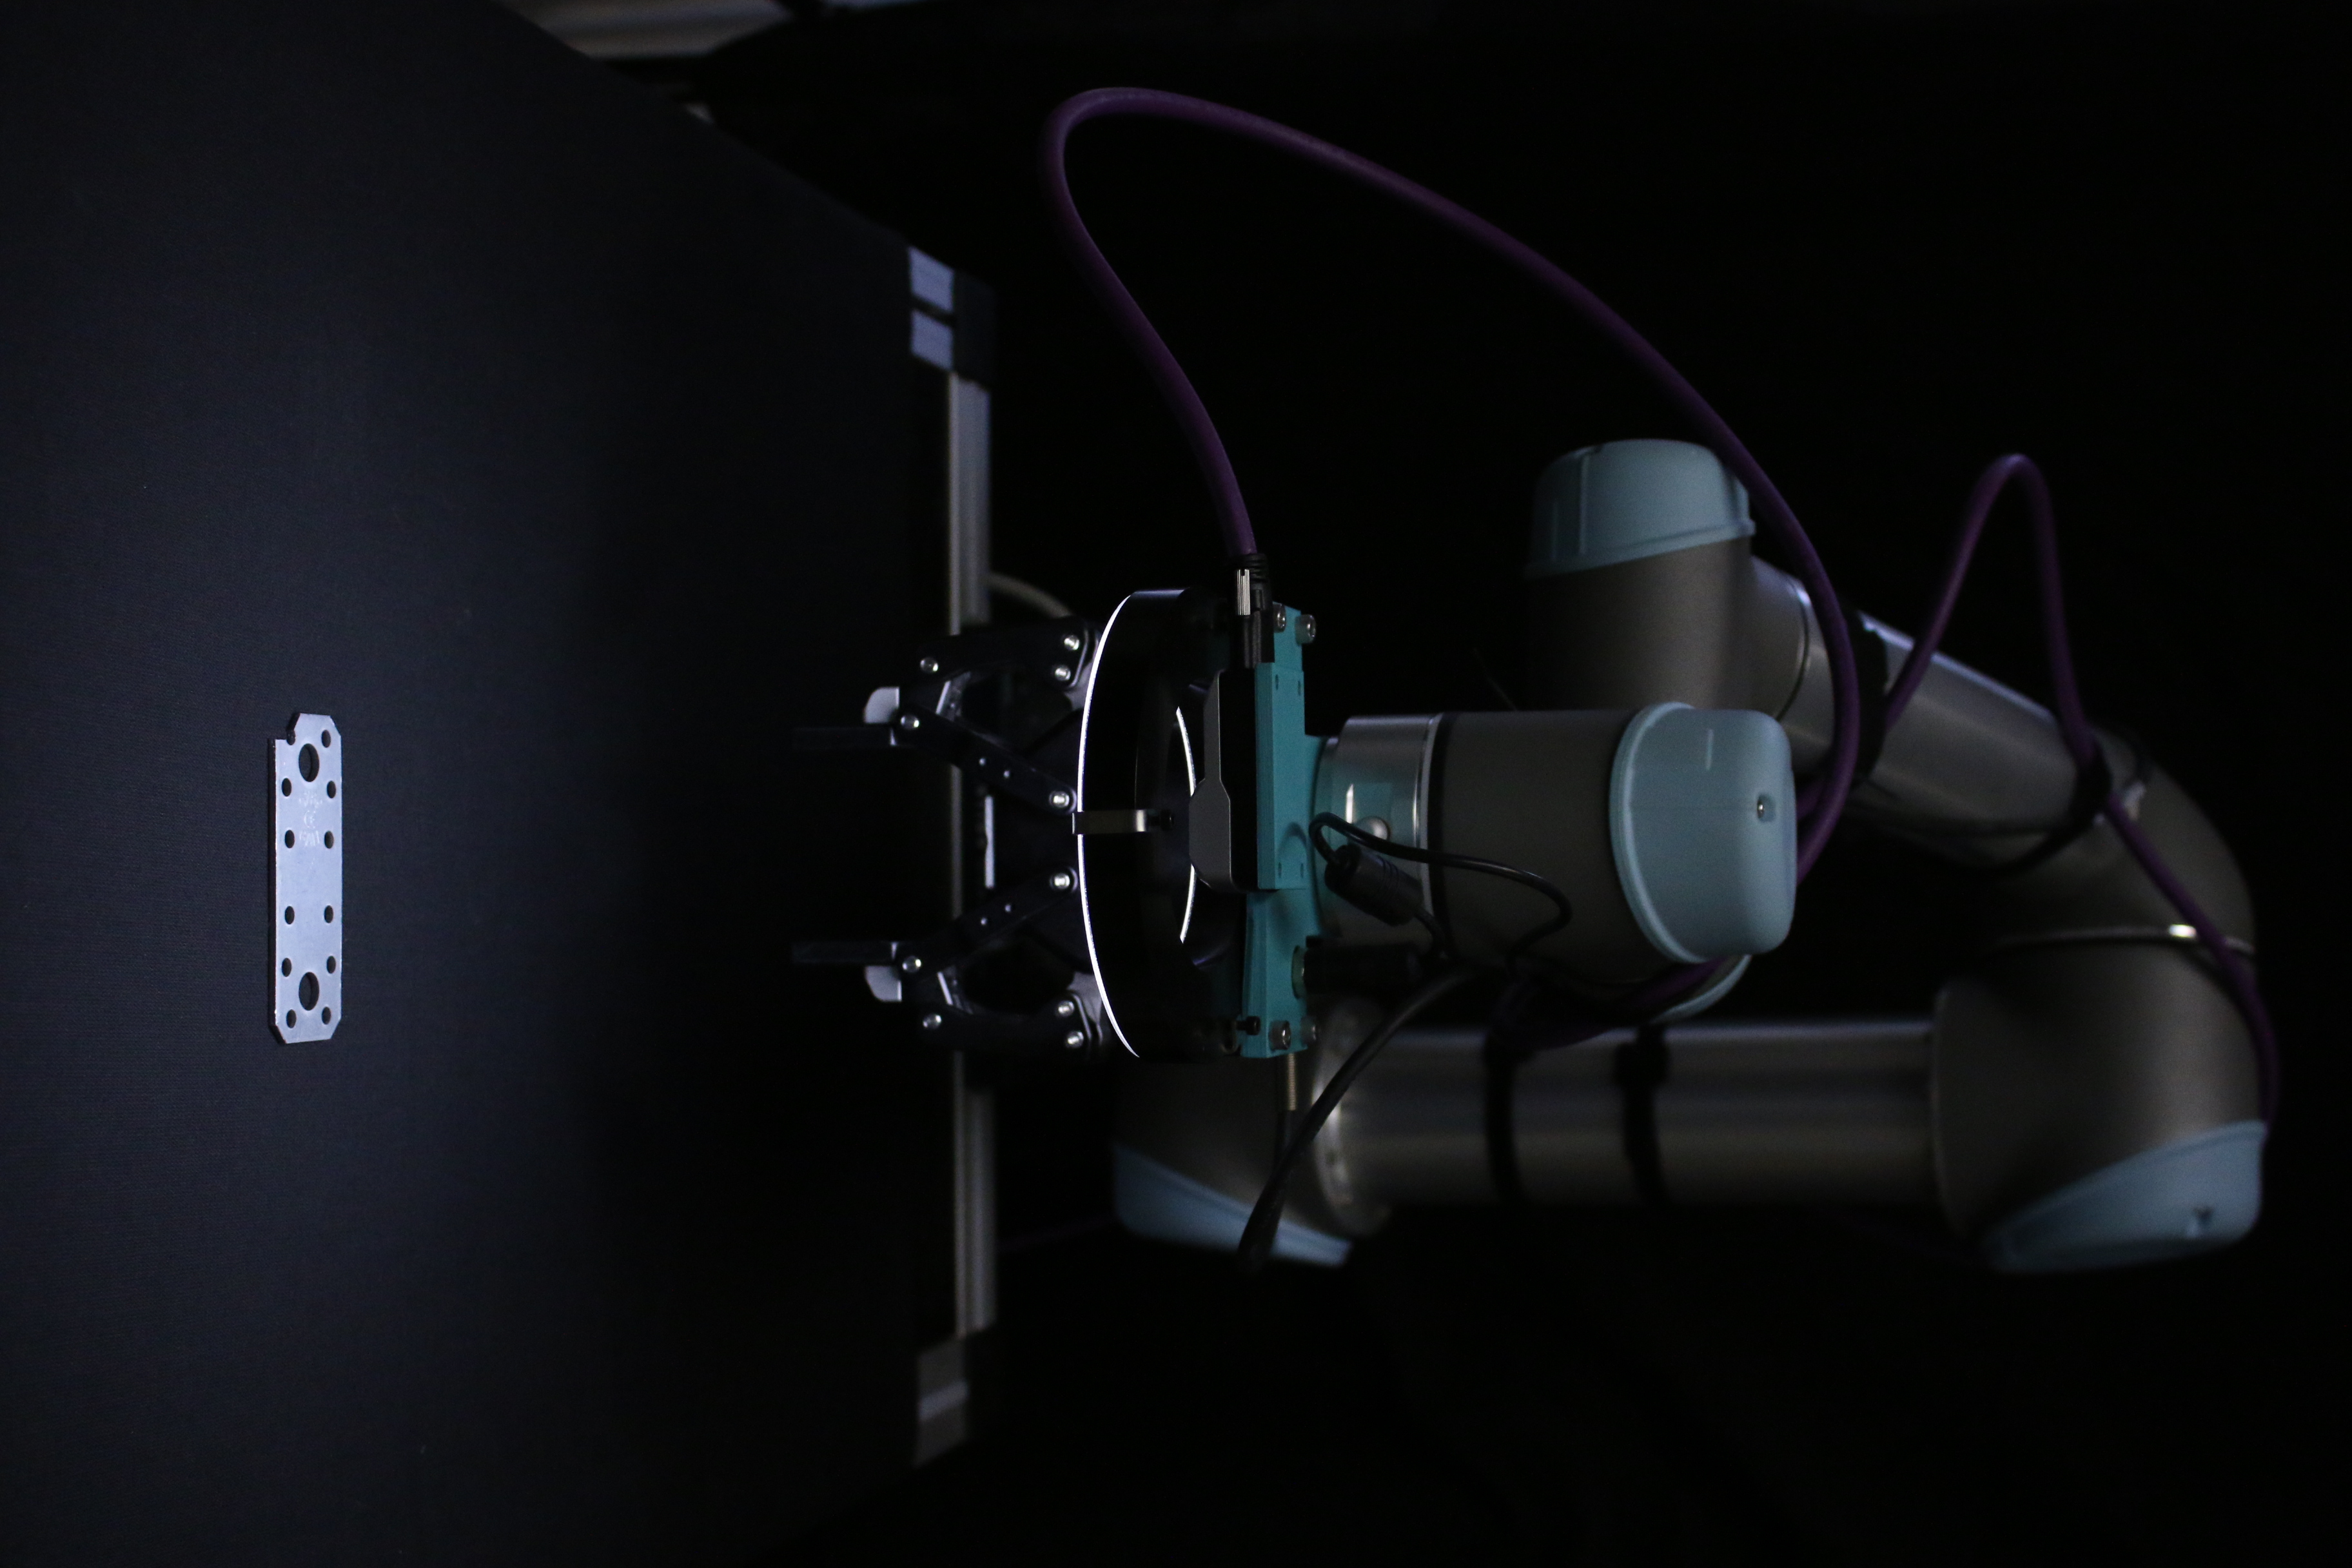
\includegraphics[angle=90, width=\textwidth]{figures/setupimages/setup_flachverbinder.JPG}
        %\caption*{Logical Anomalies}

    \end{subfigure}
    \begin{subfigure}[b]{0.3\textwidth}
        \centering
        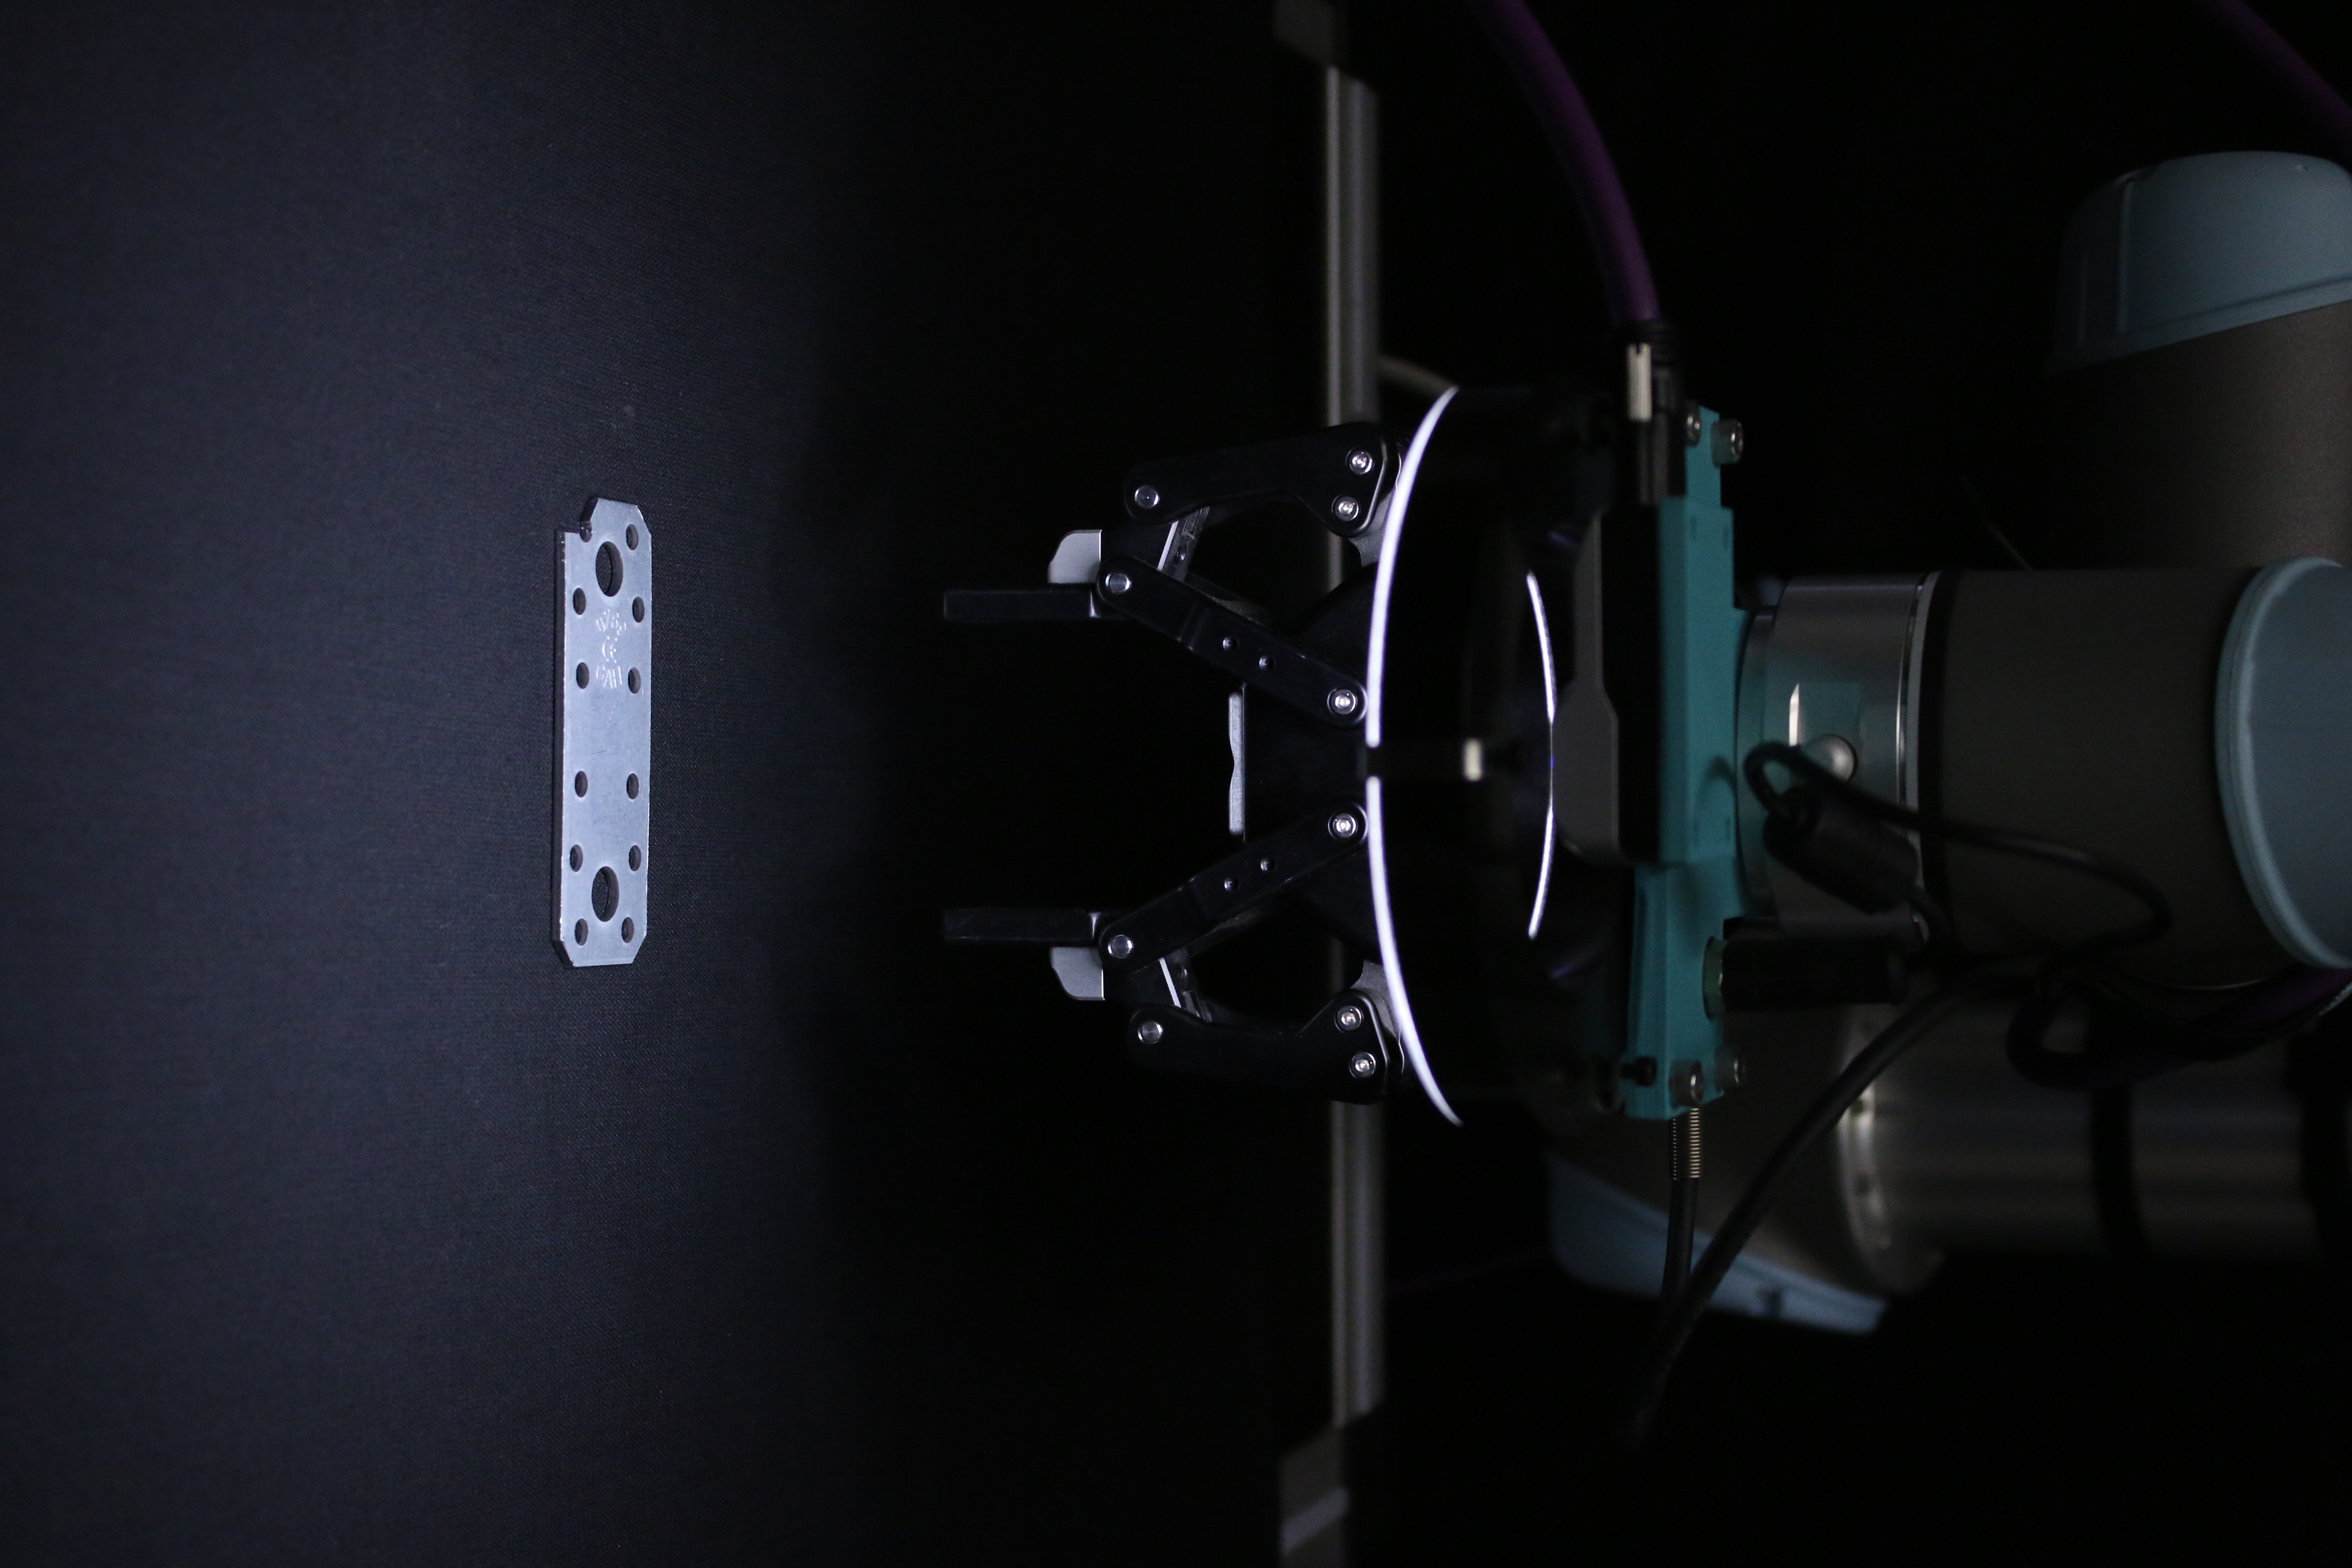
\includegraphics[angle=90, width=\textwidth]{figures/setupimages/setup_close.JPG}


    \end{subfigure}
    \caption{Manually taken images from the setup used to record the flat connector class. The images depict a wide shot of the robot mount used, 
             a closer image with a flat connector on the table and a close up of the process.}
    \label{fig:setupofdatacollection}
\end{figure}

